%%%%%%%%%%%%%%%%%%%%%%%%%%%%%%%%%%%%%%%%%
% Masters/Doctoral Thesis
% LaTeX Template
% Version 1.43 (17/5/14)
%
% This template has been downloaded from:
% http://www.LaTeXTemplates.com
%
% Original authors:
% Steven Gunn
% http://users.ecs.soton.ac.uk/srg/softwaretools/document/templates/
% and
% Sunil Patel
% http://www.sunilpatel.co.uk/thesis-template/
%
% License:
% CC BY-NC-SA 3.0 (http://creativecommons.org/licenses/by-nc-sa/3.0/)
%
% Note:
% Make sure to edit document variables in the Thesis.cls file
%
%%%%%%%%%%%%%%%%%%%%%%%%%%%%%%%%%%%%%%%%%

%----------------------------------------------------------------------------------------
%	PACKAGES AND OTHER DOCUMENT CONFIGURATIONS
%----------------------------------------------------------------------------------------

\documentclass[11pt, oneside]{Thesis} % The default font size and one-sided printing (no margin offsets)

\graphicspath{{pictures/}} % Specifies the directory where pictures are stored

\usepackage{titlesec}
\usepackage{todonotes}

\titlespacing\section{0pt}{12pt plus 4pt minus 2pt}{0pt plus 2pt minus 2pt}
\titlespacing\subsection{0pt}{12pt plus 4pt minus 2pt}{0pt plus 2pt minus 2pt}
\titlespacing\subsubsection{0pt}{12pt plus 4pt minus 2pt}{0pt plus 2pt minus 2pt}

\setlength{\footnotesep}{0.3cm}
\setlength{\skip\footins}{1cm}

\usepackage[square, numbers, comma, sort&compress]{natbib} % Use the natbib reference package - read up on this to edit the reference style; if you want text (e.g. Smith et al., 2012) for the in-text references (instead of numbers), remove 'numbers'
\title{\ttitle} % Defines the thesis title - don't touch this

%----------------------------------------------------------------------------------------
%	MAIN DOCUMENT CONTENTS AND FRONT MATTER
%----------------------------------------------------------------------------------------

\begin{document}

\frontmatter % Use roman page numbering style (i, ii, iii, iv...) for the pre-content pages

\setstretch{1.3} % Line spacing of 1.3

% Define the page headers using the FancyHdr package and set up for one-sided printing
\fancyhead{} % Clears all page headers and footers
\rhead{\thepage} % Sets the right side header to show the page number
\lhead{} % Clears the left side page header

\pagestyle{fancy} % Finally, use the "fancy" page style to implement the FancyHdr headers

\newcommand{\HRule}{\rule{\linewidth}{0.5mm}} % New command to make the lines in the title page

% PDF meta-data
\hypersetup{pdftitle={\ttitle}}
\hypersetup{pdfsubject=\subjectname}
\hypersetup{pdfauthor=\authornames}
\hypersetup{pdfkeywords=\keywordnames}

%----------------------------------------------------------------------------------------
%	TITLE PAGE
%----------------------------------------------------------------------------------------

\begin{titlepage}
\begin{center}

\vspace*{3cm}

\HRule \\[0.4cm] % Horizontal line
{\huge \bfseries \ttitle}\\ %[1cm] % Thesis title
\HRule \\[1.5cm] % Horizontal line

\Large{\textsc{Bachelor Degree Thesis}}\\[3cm] % Thesis type

\begin{minipage}[t]{0.45\textwidth}
	\begin{flushleft} \large
		\emph{Author:}\\
		\authornames % Author name - remove the \href bracket to remove the link
		\vspace{1cm}
	\end{flushleft}
\end{minipage}
\begin{minipage}[t]{0.45\textwidth}
	\begin{flushright} \large
		\emph{Supervisor:} \\
		\supname\\ % Supervisor name - remove the \href bracket to remove the link
		\emph{Department:}\\
		\textsc{\supdept}
	\end{flushright}
\end{minipage}\\[2.5cm]

\Large \textsc{\degreename}\\
\large \textit{\textsc{\major}}\\[1cm] % University requirement text
%\textit{in the}\\[0.4cm]
%\groupname\\\deptname\\[2cm] % Research group name and department name

\textsc{\large \facname}\\ % University name
\textsc{\large \univname}\\[1cm] % University name

{\large \today}\\ % Date
%\includegraphics{Logo} % University/department logo - uncomment to place it

\vfill
\end{center}

\end{titlepage}

\clearpage % Start a new page
         % Thesis title page
%----------------------------------------------------------------------------------------
%	QUOTATION PAGE
%----------------------------------------------------------------------------------------

\pagestyle{empty} % No headers or footers for the following pages

\null\vfill % Add some space to move the quote down the page a bit

\textit{``Al fin y al cabo, somos lo que hacemos para cambiar lo que somos."}

\begin{flushright}
Eduardo Galeano
\end{flushright}

\vfill\vfill\vfill\vfill\vfill\vfill\null % Add some space at the bottom to position the quote just right

\clearpage % Start a new page
         % Remarkable quotation, by someone you like
%----------------------------------------------------------------------------------------
%	ABSTRACT PAGE
%----------------------------------------------------------------------------------------

\addtotoc{Abstract} % Add the "Abstract" page entry to the Contents

\abstract{\addtocontents{toc}{\vspace{1em}} % Add a gap in the Contents, for aesthetics

The Thesis Abstract is written here (and usually kept to just this page). The page is kept centered vertically so can expand into the blank space above the title too.
}

\clearpage % Start a new page
          % Thesis abstract
%----------------------------------------------------------------------------------------
%	ACKNOWLEDGEMENTS
%----------------------------------------------------------------------------------------

\setstretch{1.3} % Reset the line-spacing to 1.3 for body text (if it has changed)

\acknowledgements{\addtocontents{toc}{\vspace{1em}} % Add a gap in the Contents, for aesthetics

First and foremost, I would like to thank Dr. Jordi Nin for his advice and guidance throughout the entire development of this project, as well as his continued support to help me achieve my present and future goals. To him and all the professors I ever had, I am grateful of their will to teach and share their knowledge and sapience with all of us students; it is a great task you carry on your shoulders and for that you have my heartfelt gratitude.

Thanks to all inLab\textit{'ers} too. There, I have grown as an engineer and, most importantly, as a person, surrounded by amazing people. Thanks to Rosa, Albert and Jaume for their guidance, and thanks to all with whom I have had the most enthralling experiences at the faculty: Albert, Anna, Carlos, Eli, Germán, Jaume, Joel, Maki, Marc, MJ, Natxo, Néstor, and sure I forget someone.

I am most thankful to my dearest friends Bernat, Borja, Laura, Natàlia, Pau; all these years have been amazing by your side. With you, life is brighter and the future is always awaiting on the horizon.

This project would not be without my family. All my gratitude and love is for my parents and my brother, who support me and raise me and teach me the most wonderful things. Thank you.

}
\clearpage % Start a new page
  % Acknowledgements (family, friends...)
%----------------------------------------------------------------------------------------
%	LIST OF CONTENTS/FIGURES/TABLES PAGES
%----------------------------------------------------------------------------------------

\pagestyle{fancy} % The page style headers have been "empty" all this time, now use the "fancy" headers as defined before to bring them back

\lhead{\emph{Contents}} % Set the left side page header to "Contents"
\tableofcontents % Write out the Table of Contents

\lhead{\emph{List of Figures}} % Set the left side page header to "List of Figures"
\listoffigures % Write out the List of Figures

\lhead{\emph{List of Tables}} % Set the left side page header to "List of Tables"
\listoftables % Write out the List of Tables
            % TABLE OF CONTENTS, figures, tables, listings...
%----------------------------------------------------------------------------------------
%	ABBREVIATIONS
%----------------------------------------------------------------------------------------

\clearpage % Start a new page

\setstretch{1.5} % Set the line spacing to 1.5, this makes the following tables easier to read

\lhead{\emph{Abbreviations}} % Set the left side page header to "Abbreviations"
\listofsymbols{ll} % Include a list of Abbreviations (a table of two columns)
{
\textbf{DR} & \textbf{D}isclosure \textbf{R}isk \\
\textbf{IL} & \textbf{I}nformation \textbf{L}oss \\
\textbf{MOA} & \textbf{M}assive \textbf{O}nline \textbf{A}nalysis \\
\textbf{SDC} & \textbf{S}tatistical \textbf{D}isclosure \textbf{C}ontrol \\
%\textbf{Acronym} & \textbf{W}hat (it) \textbf{S}tands \textbf{F}or \\
}
     % Abbreviations used throughout the thesis
%----------------------------------------------------------------------------------------
%	SYMBOLS
%----------------------------------------------------------------------------------------

\clearpage % Start a new page

\lhead{\emph{Symbols}} % Set the left side page header to "Symbols"

\listofnomenclature{lll} % Include a list of Symbols (a three column table)
{
$a$ & distance & m \\
$P$ & power & W (Js$^{-1}$) \\
% Symbol & Name & Unit \\

& & \\ % Gap to separate the Roman symbols from the Greek

$\omega$ & angular frequency & rads$^{-1}$ \\
% Symbol & Name & Unit \\
}
           % List of symbols used
%----------------------------------------------------------------------------------------
%	DEDICATION
%----------------------------------------------------------------------------------------

\setstretch{1.3} % Return the line spacing back to 1.3

\pagestyle{empty} % Page style needs to be empty for this page

\dedicatory{Dedicated to my family.} % Dedication text

\addtocontents{toc}{\vspace{2em}} % Add a gap in the Contents, for aesthetics
        % Dedication oneliner

%----------------------------------------------------------------------------------------
%	THESIS CONTENT - CHAPTERS
%----------------------------------------------------------------------------------------

\mainmatter % Begin numeric (1,2,3...) page numbering

\pagestyle{fancy} % Return the page headers back to the "fancy" style

% Include the chapters of the thesis as separate files from the Chapters folder
% Uncomment the lines as you write the chapters

\chapter{Introduction} % Main chapter title
\label{Chapter1Introduction} % For referencing the chapter elsewhere, use \ref{Chapter1Introduction}
\lhead{\emph{Introduction}} % This is for the header on each page - perhaps a shortened title

%----------------------------------------------------------------------------------------

What follows is a brief introduction to the project under review in this report and its context,
in a broad sense. The structure of this document is also outlined in the last section of this chapter.

\section{Context}
\label{Introduction::Context}

We will now provide an overview of the two main concepts that, when combined,
drive the motivation behind the inception and development of this project.

\subsection{Data mining}
\label{Introduction::Context::DataMining}

Information society produces vast amounts of data all over the world.
This data comes from innumerable sources and in diverse formats, and has been stored
for years in data warehouses, waiting to be processed. With the continuous increase
in computing power, due to the recent advances in software and hardware technologies,
the machine learning field, more commonly known as \textit{data mining}, has arisen,
allowing us to exploit this stored data and distill knowledge from it.

Data mining is, indeed, a holistic process, where many different disciplines are
involved, from data acquisition and storage, through its selection, filtering and
analysis up to information extraction, visualization and knowledge discovery.

\begin{figure}[h]
	\centering
	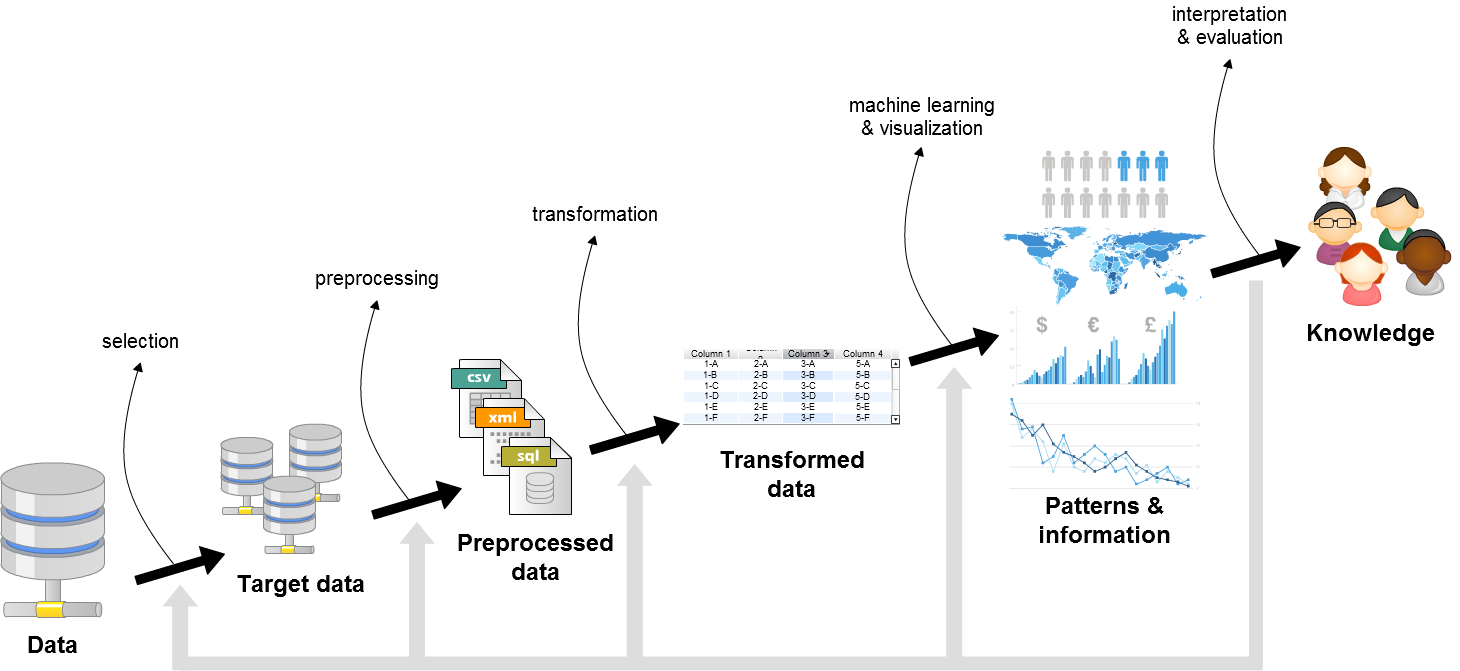
\includegraphics[width=0.9\linewidth]{figures/data-mining-process.png}
	\caption{Data mining as a process. Adapted from~\citet{Fayyad:FromDataMining}}
	\label{fig:data-mining}
\end{figure}

Data mining enables a better understanding of human or natural processes and provides
us with means to identify trends, predict future events or discover useful patterns.
Its uses range from scientific and medical applications to social sciences or business
administration~\citep{Fayyad:FromDataMining}.

\subsubsection{Facing the limits}

Despite lots of effort is put into enhancing different data mining processes, there still
are many cases where these techniques fail to perform correctly; mainly, it is a matter of scale.

On one hand, traditional data mining workflows cannot cope with the really massive
data sets that are available nowadays, if performed on a common infrastructure.
To solve this issue, clusters of hundreds or thousands of computers are used to run
such analysis. It is costly and complex but, doing so, we can mine data that we could not
some time ago.

On the other hand, we face another type of scaling problem. In some situations, data
acquisition throughput is so high that it cannot be stored anyway, so another approach
is needed to avoid the loss of information that it could deliver us. Moreover, we might
not want to store it, even when we could, but yet we want to analyze it to extract
knowledge from it, as soon as we received it. Both these scenarios are addressed with a
series of techniques known as \textit{stream mining}.

\subsubsection{Stream mining}

\textit{Stream mining} or \textit{data stream mining} is a process that allows us to
still discover knowledge and patterns in data, even when it comes in the form of a
continuous stream, or many of them~\citep{Rajaraman:MiningMassiveDatasets}. Instead of processing
all statically stored data, like traditional data mining does, a relatively small
portion of it is kept during the analysis, and it is updated when needed - either because
more resources are available to the system or because new data is acquired. A more deeper
review of this research area is given in \ref{Theory::StreamMining}.

\subsection{Privacy}
\label{Introduction::Context::Privacy}

Privacy is a concept that can be defined as the ability of an individual or group to
seclude\footnote{“Seclusion is the act of placing or keeping someone away from other people.”~\citep{web:Merriam:Seclusion}} themselves, or information about themselves, and
thereby express themselves selectively. It is understood differently depending on the social
and cultural background of each individual, but it is in fact recognised as one of the most
fundamental rights of our human nature. The Universal Declaration of Human Rights’ 12th
article~\citep{web:UN:HumanRightsDeclaration} states that:

\begin{quote}
	No one shall be subjected to arbitrary interference with his privacy, family, home or
	correspondence, nor to attacks upon his honour and reputation. Everyone has the right to
	the protection of the law against such interference or attacks.
\end{quote}

This right has been continuously violated ever since information exchange and advanced
communication technologies have been developed. Despite this did not begin with the spread
of the Internet, its adoption has greatly magnified both the ability to breach people’s privacy
and the impact that these breaches have. A more thorough analysis of privacy and its interrelations
with society and technology is given in \sref{Practical::Privacy}.

\subsection{Privacy Preserving Data Mining}
\label{Introduction::Context::PPSM}

Data mining technologies have become a relevant debate topic nowadays, concerning what
information is collected from individuals, who owns it and what are the purposes behind
its gathering. Information technologies deliver us many benefits at many levels - safer
streets, cheaper communications, better health systems, more convenient shopping - but
at the high cost of losing our privacy.

Knowledge discovery processes need data to work and, in most cases, it is sensitive and
personal. Moreover, it is massively collected and stored and analyzed without us knowing
much about it. Besides the lack of consent in this data acquisition stage of the process,
data mining poses a bigger thread on individuals: information disclosure. Sensitive data
must be treated accordingly, which involves not only good IT security practices to avoid
information leaks, but a responsible treatment when research results are published.

\subsubsection{Statistical Disclosure Control}

\textit{Statistical Disclosure Control} (SDC) is the name that the statistical community
has given to what the data mining community calls Privacy Preserving Data Mining (PPDM).
This field, whatever its preferred name is, deals with controlling that information about
specific individuals is not extracted from statistical summary results. Also, if full
datasets are to be released, PPDM methods should be applied to data in order to preserve
user's privacy, whilst maintaining the statistical significance of it, i. e., the amount
of information - knowledge - that this data can provide.

\section{The project: moa-ppsm}
\label{Introduction::moa-ppsm}

Having reviewed the main concepts to which this project is related, we can now outline
its main purpose, once we take a closer look to the technical environment in which it
will be developed.

\subsection{MOA}
\label{Introduction::moa-ppsm::MOA}

\textbf{MOA}, initials for \textbf{M}assive \textbf{O}nline \textbf{A}nalysis, is an
open source framework for data stream mining~\citep{web:MOA}, originally
developed at the University of Waikato, New Zealand. It includes several machine learning
algorithms\footnote{Algorithms used to perform the actual data mining analysis (the
“machine learning \& visualization” step on \fref{fig:data-mining}) belong to the
field of machine learning. In MOA, clustering, classification, regression, outlier
detection and recommender systems are available.} to perform the analysis and tools
to evaluate the quality of the results. It also deals with a problem known as
\textit{concept drift}\footnote{It is said of statistical properties of a target variable
being analyed, when they change over time in unforeseen ways.}. It is related to the well
known and commonly used Weka\footnote{Weka is a popular software package including
classical data mining algorithms, this is, not stream mining. It is also developed at
the University of Waikato.~\citep{web:Weka}} package, but it is built to perform at
a greater scale for more demanding problems.

\begin{figure}[h]
	\centering
	
\includegraphics[width=0.4\linewidth]{figures/moa-logo.jpg}
	\caption{Massive Online Analysis logo.}
	\label{fig:moa-logo}
\end{figure}

\subsubsection{MOA filters}

One of the available features in MOA is the use of \textit{filters}, which can process
streaming data before or after being fed to other systems or algorithms, such as learners
or file writers. However, few filters are currently shipped within the latest MOA distribution,
namely a filter to replace \textit{missing values}\footnote{In statistics, missing data, or missing values,
occur when no data value is stored for the variable in an observation. Missing data are a
common occurrence and can have a significant effect on the conclusions that can be drawn
from the data.} and a filter that adds noise to data.

\subsubsection{MOA extensions}

When working with MOA, the environment consists of the core library, but \textit{extensions}
can be used to enhance the existing methods or to provide additional features, based on
the core tools that MOA already provides. A series of extensions have been developed and can
be found on MOA's website, at \url{http://moa.cms.waikato.ac.nz/moa-extensions}.

\subsection{The project in a nutshell}
\label{Introduction::moa-ppsm::ProjectNutshell}

Summing up, the aim of this project is to \textbf{implement privacy preserving filters
for the MOA stream mining framework}. This is, adapt some well-known SDC methods to a stream mining environment and, more precisely, to the MOA software framework, in the form of a MOA extension.

\section{Report structure}
\label{Introduction::Structure}

The structure of this report is meant to give an overview of the development process of the project, from the theoretical foundations that are necessary to understand the work to the final results and conclusions.

\cref{Chapter2TheoreticalFramework} covers the theory basis behind the SDC methods implemented in the project and provides some insights on different stream mining approaches. \cref{Chapter3StateOfTheArt} discusses state of the art solutions concerning SDC for static databases (not streaming data). \cref{Chapter4PracticalAspects} analyzes more thoroughly the motivation behind privacy-preserving data mining by discussing \textit{practical} questions like the relationship between society and privacy or the legal framework that applies to the context of this project. Project management is layed out in \cref{Chapter5ProjectManagement} and then the report turns to more technical related topics, such as implementation details and desgin decisions, covered in \cref{Chapter6ImplementingFilters}, as well as benchmarking, in \cref{Chapter7Benchmarking}. Finally, the report and project conclusions are given in \cref{Chapter8conclusions}, covering both achievements and possible future work.

\chapter{Theoretical framework} % Main chapter title
\label{Chapter2TheoreticalFramework} % For referencing the chapter elsewhere, use \ref{Chapter1Introduction}
\lhead{\emph{Theoretical framework}} % This is for the header on each page - perhaps a shortened title

%----------------------------------------------------------------------------------------

\todo{write an appropriate intro to theoretical framework}
What follows is a brief introduction to the project under review in this report and its context,
in a broad sense. The structure of this document is also outlined in the last section of this chapter.

\section{Stream Mining}
\label{Theory::StreamMining}

Data stream mining is a relatively new field. Even though its theoretical foundation is based in well-established statistical and computational approaches, it has not been until recent years that this research area has experimented a great growth in interest.

The main problem when dealing with streaming data is the high throughput of data being analyzed, under computational resources constraints. Variable data rates is another problem that has to be addressed too. Once these problems are resolved, the same kind of data mining analysis as in the case of batch data processing are available: classification, regression or clustering tasks, as well as outlier detection and recommendation systems. We will not cover these techniques here, because they are not related to this project, by themselves. Instead, we will have a look at some different stream mining solutions, because their working principles do affect the way the project’s algorithms will be implemented.

\subsection{Stream mining approaches}
\label{Theory::StreamMining::Approaches}

Solutions provided in this field can be categorized into \textit{data-based} and \textit{task-based} ones~\citep{Gaber:MiningDataStreamsReview}, depending on their approach.

\subsubsection*{Data-based stream mining solutions}

The idea behind these solutions is to use a subset of the original dataset to perform the required analyses. Diverse techniques that have been used in this sense can further be split into two more categories:

\begin{itemize}
	\item \textbf{Sampling methods:} either by randomly picking samples of the data stream or by randomly selecting chunks (subsets) of the stream, sampling methods discard part of the incoming data, while performing the knowledge discovery processes with the sampled data. The main problem with this approach is that is hard to know when to pick a sample or which records should be stored, because there is no previous knowledge of the dataset size or its information structure.

	\item \textbf{Summarizing methods:} they use aggregated data or calculated statistical measures (that are continuously recalculated) to provide the information needed for the data mining algorithms. In this case, it is the loss of information and accuracy and the inability to control data distribution fluctuations what renders these methods not so usable as it was desired.
\end{itemize}

\begin{figure}
\centering
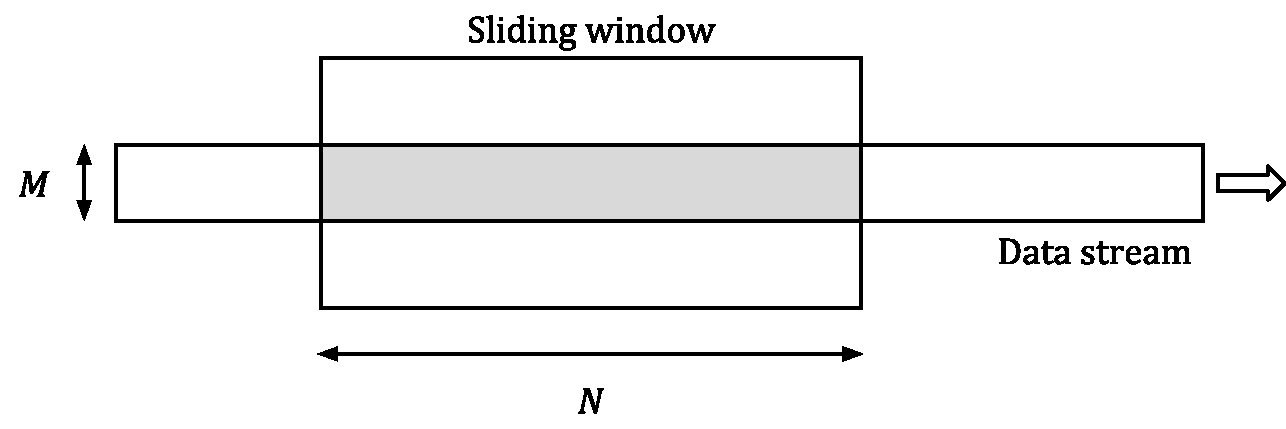
\includegraphics[width=0.9\linewidth]{figures/sliding-window.pdf}
\caption[Sliding window based stream processing.]{Processing a data stream using a \textit{sliding window} approach. In the figure, $N$ is the \textit{size} of the sliding window, in terms of the number of samples of the stream being stored, whereas $M$ is the number of \textit{attributes} of the samples in the stream.}
\label{fig:sliding-window}
\end{figure}

\subsubsection*{Task-based stream mining solutions}

The solutions that fall into this category are based not on performing data transformations, but on changing the data mining methods to enable their use on data streams.

\begin{itemize}
	\item \textbf{Approximation algorithms:} these are a kind of algorithms that are designed to solve computationally hard problems, by giving an approximate result. Instead of computing exact solutions, they just guarantee a certain error bound. The problem with these methods is, again, the high received data throughput, which they cannot cope as well. Additional tooling is therefore needed if one wishes to use them.

	\item \textbf{Sliding window method:} this method, a common pattern in many online\footnote{In computer science, an \textit{online algorithm} is one that can process its input piece-by-piece in a serial fashion, i.e., in the order that the input is fed to the algorithm, without having the entire input available from the start.} applications, maintains a \textit{sliding window} in which the most recent data is kept. As data is received from the incoming streams, this window “advances” so new observations are kept inside, as can be seen in \fref{fig:sliding-window}. The data mining analyses are then performed using the data available inside the window and summarized versions of the older records, in the form of statistical measures or aggregated data.
	This particular method is the one that the MOA package uses - thus its name: Massive \textbf{Online} Analysis. This solution scheme enables dealing with concept drift, which would not be possible if just aggregated data was used.

	\item \textbf{Algorithm output granularity:} this method is a resource-aware data analysis approach that can perform the local analysis on resource constrained devices, by adapting to resource availability and data stream rates - when resources are completely running out, the results are merged and stored.
\end{itemize}

\section{Statistical Disclosure Control}
\label{Theory:SDC}

As was already introduced in \sref{Introduction::Context::PPSM}, the purpose of Statistical Disclosure Control (SDC) is to prevent confidential information from being linked to specific individuals to whom this data belongs. We will review now some concepts related to data disclosure and SDC methods and some theoretical foundations.

\subsection{Privacy preserving algorithms} 
\label{Theory:SDC:Algorithms}

As a quick and superficial review, the algorithms\footnote{We will not cover every algorithm in detail, because some of them are not included in the scope of this project.} being used nowadays to achieve effective privacy preserving in datasets can be categorized into the following groups~\cite{Hundepool:StatisticalDisclosureControl}:

\begin{itemize}
	\item \textit{Non-perturbative data masking:} these kind of methods do not perform data values transformations. Instead, they are based in partial suppressions of records or reductions of detail of the datasets. Some examples are:
	\begin{itemize}
		\item Sampling
		\item Global recoding
		\item Top and bottom coding
		\item Local suppression
	\end{itemize}

	\item \textit{Perturbative data masking:} these methods do release the whole dataset, if required, but it is perturbed, this is, values are changed by adding them noise. This way, records are diffused and reidentifying individuals is harder. Some examples are:
	\begin{itemize}
		\item Noise masking
		\item Micro-aggregation
		\item Rank swapping
		\item Data shuffling
		\item Rounding
		\item Re-sampling
		\item PRAM
		\item MASSC
	\end{itemize}
\end{itemize}

\subsection{Disclosure \& types of variables}
\label{Theory:SDC:DisclosureTypes}

When assessing the disclosure risks of a given dataset (or data stream) we must have a look at the different kind of variables this data is composed of. We will stick to a classic~\citep{Templ:IntroSDC} categorization of such attributes into three groups, which need not be disjunctive, as follows:

\begin{itemize}
	\item \textbf{Identifiers:} variables that precisely identify individuals, e.g., social insurance numbers, person names, or addresses.
	\item \textbf{Quasi-identifiers:} a set of variables that, when considered together, can be used to identify individual units. It might be possible to, for example, identify people by combining variables such as gender, age, region and occupation.
	\item \textbf{Non-identifying variables:} these are neither \textit{identifiers} nor \textit{quasi-identifiers}.
\end{itemize}

Concerning \textit{disclosure}, it is also defined differently depending on the type of privacy breach that has occurred:

\begin{itemize}
	\item We talk about \textit{identity disclosure} when a specific individual record can be recognised in a dataset, i.e., when linkage with external available data is possible. Identity disclosure is performed using direct identifiers, rare combinations of values in quasi-identifier attributes and exact knowledge of variable values in external databases.
	\item In the case of \textit{attribute disclosure}, the intruder is able to gather sensitive information about a specific unit from the released data, where it is directly available. For example, if no perturbation is applied to the original values of the \textit{wages} variable, one could learn how much a person is earning if its identity is disclosed too.
	\item \textit{Inferential disclosure}, the most general case, occurs when an intruder is able to, with some uncertainty, predict or \textit{infer} confidential information about an individual from the statistical properties of data.
\end{itemize}

It is important to remark that a subset of critical variables might be exploited to disclose every information about a single unit in a dataset. Thus, we are bound to carefully select which variables of the dataset might be released to further users of the data, while trying to maximize its statistical utility. More concretely, it is extremely important to \textbf{not release identifiers} and to analyze quasi-identifiers closely, in order to avoid information leaks and privacy breaches.

\subsection{Disclosure Risk}
\label{Theory:SDC:DiscRisk}

Concerning the safety of the released data, \textbf{Disclosure Risk} (DR) is a common way to measure and assess the risk of re-identification of particular individuals. Re-identification happens when some sensitive and confidential data that have been released are subsequently linked to a particular individual, which results in a confidentiality breach. There are a number of different approaches in how to assess disclosure risk and whether to measure it \textit{per record} or globally, taking into account the whole dataset.

As noted in \citep{Domingo:DiscRiskAssessment}, there is not much literature on disclosure risk that can be used for a broad class of perturbative methods; disclosure risk measures tend instead to be method-specific. Therefore, empirical methods are most used to assess disclosure risk for these kind of methods.

\subsubsection{Record linkage}

Most notably, the mechanisms used to measure disclosure risk follow a \textit{record linkage} approach. This is, after an SDC method has been used to anonymize data, a record linkage procedure is applied to the original and released (masked, anonymized) datasets. This \textit{linkage} attempts to identify, for each record in the masked dataset, which is the corresponding record in the original dataset. If such correspondance is verified, the record is labeled as \textit{correctly linked}. A generic measure for disclosure risk is the percentage of correctly linked records from the total amount in the dataset.

\begin{itemize}
	\item \textbf{Distance-based record linkage:} provided that a \textit{distance} measure can be defined between the original and the masked datasets, linkage is performed as follows: for each record in the anonymized dataset, a distance to each record in the original dataset is calculated. The nearest record, in terms of this distance measurement, is assumed to be the corresponding record, thus establishing a \textit{link} between them. This linkage is then verified to assess how many of these guesses are true re-identifications.
	
	\item \textbf{Probabilistic record linkage:} in this case, the matching algoritm works a little different. For each possible pair of original and masked records, a \textit{coincidence vector} is defined. This vector holds, for each attribute, whether or not the values of the considered records are equal. An index is computed afterwards over these vectors and, using such index, the records pairs are classified as \textit{linked} or \textit{not linked}. Again, this linkage is verified to assess the number of true re-identifications.
\end{itemize}

\subsection{Information Loss}
\label{Theory:SDC:InfoLoss}

Another key measurement concerning data protection is \textbf{Information Loss} (IL) or \textit{data utility}, which could be defined as the amount of useful statistical information that is lost along the data masking process. A good SDC method should try to minimize IL, in order to provide optimally useful data to the legitimate users of such data, while also keeping a low disclosure risk. It is important to note that these two properties are inversely proportional: the lower disclosure risk is, the higher information loss will occur. This trade off between these two parameters is often a difficult and challenging task and should be taken into very careful consideration, depending on the release policies that apply, the kind of data being released and the sensitivity of the information contained in such data. This evaluation should be performed not only from a purely quantitave and numerical point of view, but from an ethical and privacy concerned one too.

As well as with disclosure risk, a number of methods and approaches are taken to assess information loss when releasing privacy protected datasets, ranging from unbounded~\citep{Domingo:SDCMethodsInfoLoss} to probabilistic (bound to the $[0,1]$ interval) measurements~\citep{Mateo:ProbInfLossMeasures}.

\subsubsection*{Unbounded Information Loss}

An example framework to assess IL was given in \citep{Domingo:SDCMethodsInfoLoss}, which evaluates some key statistical properties of the released data. More concretely, it computes three \textit{discrepancy} measurements for a series of pairs of matrices (correlation, covariance, etc. of the original and masked datasets), namely the \textit{mean square error}, the \textit{mean absolute error} and the \textit{mean variation}.

\subsubsection*{Probabilistic Information Loss}

The aim of measuring IL in a probabilistic manner is to bound this measurement to the $[0,1]$ range, thus allowing its comparison with DR, which is also generally expressed within this range. This way, a \textit{score} could be calculated from both normalized measures for an SDC method, easing parameters selection to data protectors, for example.

\subsection{Privacy guarantees}
\label{Theory:SDC:Guarantees}

Many different methods have been developed to help prevent information disclosure when data mining datasets or results are released. These algorithms pursue the generation of results or data that have particular properties concerning privacy preservation. Some of the desirable properties of privacy-protected data are described in the following sections, but no formal definition is provided for some of them (please refer to the original papers and publications to understand them better).

\subsubsection{\textit{k}-Anonymity}

First described in 2002, by Latanya Sweeney, a release of data is said to have the \textit{$k$-anonymity} property if the information for each person contained in the release cannot be distinguished from at least $k-1$ individuals whose information also appears in the release~\citep{Sweeney:kAnonymity}. A more formal definition uses the previously reviewed concept of \textit{quasi-identifiers} (see~\sref{Theory:SDC:DisclosureTypes}).

\begin{definition}~($k$-Anonymity)
A dataset is said to satisfy $k$-anonymity for an integer $k > 1$ if, for each combination of values of quasi-identifiers, at least $k$ records exist in the dataset sharing that combination.~\citep{Domingo:EnhancingDiffPrivMicroaggregation}
\end{definition}

An intruder trying to use a $k$-anonymous dataset to do, for example, record linkage against an external source of information will find that at least $k$ records in the dataset match any value of the quasi-identifiers that he or she is trying to use to perform the linkage. Thus, re-identification is limited to \textit{groups}, this is, no individual records can be linked, just groups of size at least $k$.

\subsubsection{\textit{l}-Diversity}

The evolution of the concept of $k$-anonymity is \textit{$l$-diversity} and adds further privacy preservation by adding intra-group diversity, so to avoid the flaws of the $k$-anonymity privacy model~\citep{Machanavajjhala:lDiversity}.

\subsubsection{\textit{t}-Closeness}

Further on, the \textit{$t$-closeness} property definition adds attribute-based privacy enforcement to the $l$-diversity model: to better preserve privacy, all values (all observations) from a particular attribute must not be too much different - instead, they should be close up to a certain threshold~\citep{Ninghui:tCloseness}. This is needed to preserve the privacy of those records that are more easily identifiable because their attribute values are more distinguishable.

\subsubsection{Differential Privacy}

Described in~\citet{Dwork:DifferentialPrivacy}, \textit{differential privacy} is a condition \textit{on the release mechanism} (not the dataset) that guarantees a strong privacy preservation level for some particular data uses contexts. Differential privacy is introduced in an \textit{interactive} setting, i.e., in a query-response data retrieval environment, and offers probabilistic guarantees that the contribution of any single individual to thenquery response is limited.

\begin{definition}~($\varepsilon$-Differential privacy)
A randomized mechanism\footnote{By \textit{mechanism}, we refer to any kind of function or system used to query for data.} $\mathcal{M}$ gives $\varepsilon$-differential privacy if, for all datasets $X_1$, $X_2$ such that one can be obtained from the other by modifying a \textit{single} record, and all $S \subset Range(\mathcal{M})$, it holds
\begin{equation}
P(\mathcal{M}(X_1) \in S) \leq \mathrm{exp}(\varepsilon) \times P(\mathcal{M}(X_2) \in S)
\end{equation}
\end{definition}

This definition, cited from~\citet{Domingo:EnhancingDiffPrivMicroaggregation}, easier to understand than the original one given in~\citet{Dwork:DifferentialPrivacy}, states that, given an $\varepsilon$-differential privacy mechanism $\mathcal{M}$ and any possible output $r$, the presence or abscence of a participant (in terms of the dataset, a \textit{row}) will cause at most a multiplicative $e^\varepsilon$ change in the probability of the mechanism to output a response $r$.
\section{SDC methods}
\label{Theory:SDCMethods}

We will describe now some of the most common methods and mechanisms used in SDC applications to anonymize data or provide privacy preserving data releases.

\subsection*{Notation}

We assume the following notation for the subsequent method descriptions:

\begin{itemize}
	\item
	The original dataset is the matrix $X$, with $n$ rows (samples) and $m$ attributes or variables. Therefore, the $x_{ij}$ element of the dataset denotes the value that the $j$-th attribute takes in the $i$-th row for any $1 \leq i \leq n$ and $1 \leq j \leq m$.
	
	\item
	The anonymized (protected) dataset is named $X'$.
\end{itemize}

\subsection{Noise Addition}
\label{Theory:SDCMethods:NoiseAddition}

Noise addition or \textit{additive noise masking} is a fairly simple method that is based on the addition of gaussian noise to data, thus randomly distorting its values and difficulting re-identification of individuals. The main additive noise algorithms in the literature are~\citep[p. 54]{Hundepool:StatisticalDisclosureControl}:

\begin{itemize}
	\item
	Uncorrelated noise addition.
	\item
	Correlated noise addition.
	\item
	Noise addition and linear transformation.
	\item
	Noise addition and non-linear transformation.
\end{itemize}

We will only cover the first couple of methods, because of the inherent difficulty of the latter, both in its theoretical basis and its practical implementation, which renders them not suitable for the needs of this project.

\subsubsection{Uncorrelated noise addition}

Masking by additive noise the $j$-th variable of an original dataset $X$ yields an anonymized dataset $X'$ such that

\begin{equation}
x_{ij}' = x_{ij} + \epsilon\ \ \ \text{for}\ 1 \leq i \leq n
\end{equation}

where $\epsilon$ is drawn from a random variable $\varepsilon_j \sim N(0,\sigma_{\varepsilon_j}^2)$. The general assumption is that the variances of each $\varepsilon_j$ are proportional to those of the original variables, this is, if $\textrm{Var}(X_j) = \sigma_j^2$ is the variance of the $j$-th attibute of the dataset $X$, then $\sigma_{\varepsilon_j}^2 := \alpha\sigma_j^2$.

While this method preserves means and covariances, it is, unfortunately, not able to preserve variances nor correlation coefficients.

\subsubsection{Correlated noise addition}

This method is aimed to also preserve correlation coefficients, with respect to \textit{uncorrelated} noise addition. The main difference with the previous mechanism is that the covariance matrix of the errors is now proportional to the covariance matrix of the data: $\varepsilon \sim N(0,\Sigma_\varepsilon)$, where $\Sigma_\varepsilon = \alpha\Sigma$.

Masking by correlated noise addition provides data with higher analytical utility than masking using uncorrelated noise, as long as $\alpha$ is revealed to the data user. However, the low level of protection yielded by this method and the previous one render them as not very useful for truly important SDC applications.

\subsection{Microaggregation}
\label{Theory:SDCMethods:Microaggregation}

Originally described for continuous (numerical) data, microaggregation is a family of SDC methods that, in the most general form, consist of making homogeneous groups of $k$ or more individuals (rows) from within the $X$ dataset to later replace their values with aggregated ones, this is, averages, computed on the groups themselves. These grouped and aggregated records conform the resulting $X'$ release dataset.

Two main approaches are taken when considering microaggregation techniques: \textit{univariate} and \textit{multivariate} microaggregation. The difference remains in the number of variables used to perform the \textit{clustering} phase of the method: a single variable and multiple attributes, correspondingly. As can be assessed in the literature, the univariate approach causes either a very high information loss or a very high disclosure risk, thus not being appropriate for normal SDC uses~\citep[p. 63]{Hundepool:StatisticalDisclosureControl}. On the other hand, multivariate microaggregation, proposed by~\citet{Domingo:PracticalMicroaggregation}, is considered an excellent protection method and, as such, we will focus on this approach.

It is important to note that this family of techniques are directly related to $k$-anonymity, as proved in~\citet{Domingo:KAnonMicroagg}.

\subsubsection{Partition}

The first and most computational complex task to do in a microaggregation method is to partition the dataset into $g$ groups of size at least $k > 1$, which is, indeed, a \textit{clustering} task. This proves to be quite difficult, but an optimal solution approximation with respect to information loss was already given in~\citep{Domingo:KAnonMicroagg} and further refined in~\citet{Domingo:MuAproxPolyTimeMicroagg}.

The aim of these partition methods is to find the optimal $k$-partition that maximizes within-group homogeneity. Following~\citet{Domingo:PracticalMicroaggregation}, a practical information loss measure for microaggregation, relatively common in the clustering literature, is the ratio of within-group homogeneity over the total sum of squares (the sum of \textit{within} and \textit{between} group homogeneity)

\begin{equation}\label{eq:clustering-info-loss}
L = \frac{SSE}{SST}
\end{equation}

The within-group homogeneity ($SSE$) is defined as

\begin{equation}
SSE = \sum_{i=1}^{g} \sum_{j=1}^{n_i} (x_{ij} - \mathbf{\bar{x}_i})^2
\end{equation}

where $g$ denotes the total number of groups of $n_i$ elements each and $\mathbf{\bar{x}_i}$ denotes the $i$-th group centroid. The between-groups sum of squares, $SSA$, is

\begin{equation}
SSA = \sum_{i=1}^{g} n_i (\mathbf{\bar{x}_i} - \mathbf{\bar{x}})^2
\end{equation}

where $\mathbf{\bar{x}}$ is the average vector over the whole dataset. The total sum of squares is, then, $SST = SSE + SSA$.

Because microaggregation replaces values in a group by the group centroid, if we recall~\eref{eq:clustering-info-loss}, it follows that the higher the within-group homogeneity, the lower the information loss is. Both the MDAV~\citep{Domingo:KAnonMicroagg} (Maximum Distance to Average Vector) and $\mu$-Approx~\citep{Domingo:MuAproxPolyTimeMicroagg} algorithms are built to partition the dataset into groups, while minimizing information loss, exploiting the previous theoretical result.

\subsubsection{Aggregation}

The aggregation step is the simplest of the ones that take place in a microaggregation setting: for each group $g$ of at least $k$ records and for each attribute $1 \leq j \leq m$, an \textit{aggregate} $\gamma$ is computed among the values of the $j$-th variable for the records in the group. This aggregate is then imputed to each record for its $j$-th attribute.

Concerning the types of variables that are aggregated~\citep{Domingo:KAnonMicroagg}:

\begin{itemize}
	\item
	\textbf{Continuous attributes:} the aggregated value correponds with the arithmetical mean of the selected values.
	\item
	\textbf{Categorical attributes:} the aggregated value should either be the median or the mode of the selected values.
\end{itemize}

\subsection{Rank Swapping}
\label{Theory:SDCMethods:RankSwapping}

%TODO
\todo{rank swapping}

\subsection{Laplacian Mechanism}
\label{Theory:SDCMethods:LaplacianMechanism}

%TODO
\todo{Laplacian}

\chapter{State of the art} % Main chapter title
\label{Chapter3StateOfTheArt} % For referencing the chapter elsewhere, use \ref{Chapter1Introduction}
\lhead{\emph{State of the art}} % This is for the header on each page - perhaps a shortened title

%----------------------------------------------------------------------------------------

This chapter gives further insights concerning the latest discoveries and cutting-edge technological solutions related to the main knowledge fields that affect this project: \textit{data stream mining} and \textit{statistical disclosure control}.

\section{Stream mining software}
\label{State::StreamMining}

Data stream mining is a relatively new field. Even though its theoretical foundation is based in well-established statistical and computational approaches, it has not been until recent years that this research area has experimented a great growth in interest~\citet{Gaber:MiningDataStreamsReview}.

Because it is an incipient field, stream mining software packages are quite uncommon. Even though specific applications have been developed (see~\citet{Kargupta:MineFleet}), MOA remains as one of the few generic, free and open sourced systems. One example of a commercial solution that includes support for data stream mining is RapidMiner, through the use of plugins. 

MOA is currently the most complete framework for data stream clustering research and it is an important pioneer in experimenting with data stream algorithms. MOA's advantages are that it interfaces with WEKA, provides already a set of data stream classification and clustering algorithms and it has a clear Java interface to add new algorithms or use the existing algorithms in other applications.

Related to MOA, a new project called SAMOA (from Scalable Advanced Massive Online Analysis) is being developed too, based on MOA itself and a couple of streaming processing engines: Apache S4~\citep{web:ApacheS4} and Apache Storm~\citep{web:ApacheStorm}, developed by the Apache Software Foundation.

Finally, an R package called \texttt{stream} was released into the CRAN repository\footnote{The capabilities of the R language are extended through user-created packages. Most of these packages are available at the Comprehensive R Archive Network (CRAN), on the following web address: \url{http://cran.r-project.org}.} in 2013. It allows to do real time analytics on data streams and is currently focused on clustering algorithms available in MOA.

\subsection{The MOA framework}

Massive Online Analysis (MOA) is a software environment for implementing algorithms and running experiments for online learning from evolving data streams. MOA is designed to deal with the challenging problems of scaling up the implementation of state of the art algorithms to real world dataset sizes and of making algorithms comparable in benchmark streaming settings.

MOA contains a collection of offline and online algorithms for both classification and clustering as well as tools for evaluation. Researchers benefit from MOA by getting insights into workings and problems of different approaches, practitioners can easily compare several algorithms and apply them to real world data sets and settings.

\begin{figure}
\centering
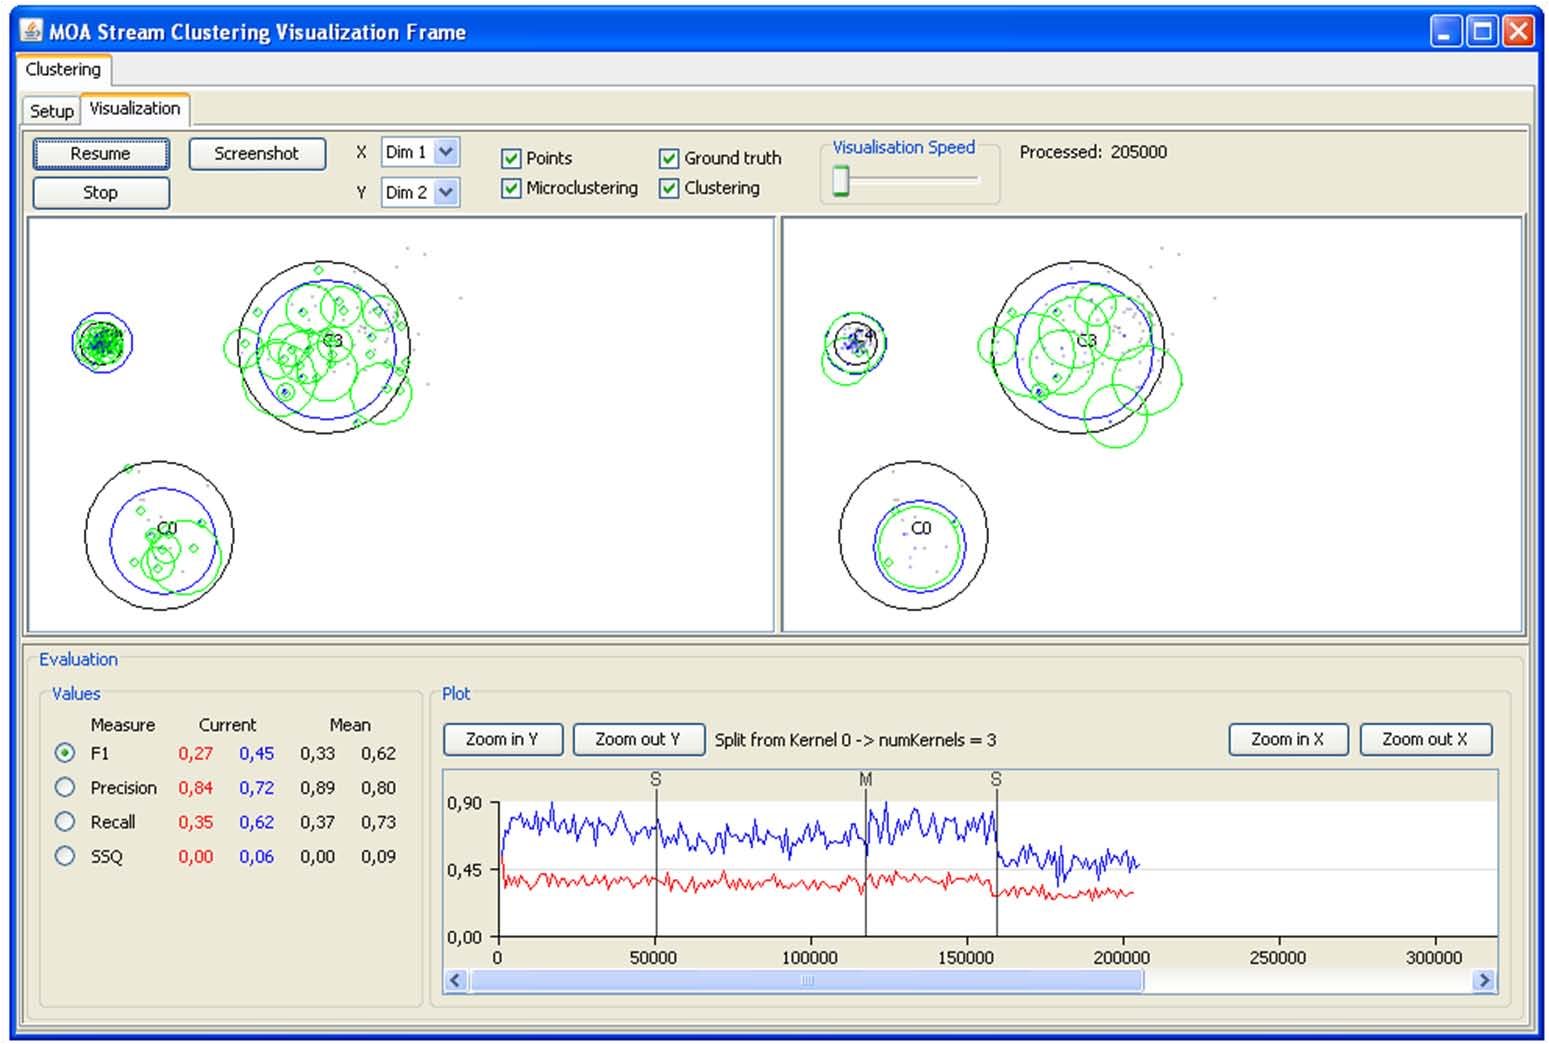
\includegraphics[width=0.8\linewidth]{figures/moa-gui-2.png}
\caption[MOA's Graphical User Interface]{MOA's Graphical User Interface, showing the clustering visualization capabilities of the software.}
\end{figure}

MOA supports bi-directional interaction with WEKA, the Waikato Environment for Knowledge Analysis, which is an award-winning open-source workbench containing implementations of a wide range of batch machine learning methods. WEKA is also written in Java. The main benefits of Java are portability, where applications can be run on any platform with an appropriate Java virtual machine, and the strong and well-developed support libraries. Use of the language is widespread, and features such as the automatic garbage collection help to reduce programmer burden and error.

The MOA framework provides a graphical user interface (GUI), which eases its use, when experiments can be carried out using the algorithms already included in the framework. However, for more complicated analysis or industry-scaled uses, MOA offers the possibility to be used using a command line interface, which is extremely powerful and flexible. Also, due to its open source nature and the fact that it is built in Java, custom procedures and integration techniques can be developed to meet the data analysis requirements. Last but not least, when the core features are not sufficient for the user's needs, MOA can be extended with new mining algorithms, new stream generators or evaluation measures, like the SDC filters that we will implement in this project.
\section{Statistical Disclosure Control software}
\label{State::SDC}



\textbf{Privacy preserving \textit{Stream} Mining:} many of the previously listed methods are already implemented in many classical data mining frameworks and software systems; for example, the \texttt{sdcMicro} package for the \textbf{R} statistical package~\cite{sdcMicro}. However, privacy preserving methods are still not widespread in the stream mining ecosystem - that is another motivation for this project.


\chapter{Practical aspects} % Main chapter title
\label{Chapter4PracticalAspects} % For referencing the chapter elsewhere, use \ref{Chapter1Introduction}
\lhead{\emph{Practical aspects}} % This is for the header on each page - perhaps a shortened title

%----------------------------------------------------------------------------------------

This chapter addresses the \textit{practical} aspects of this project, this is, those that are related to the \textit{praxis}\footnote{\textit{Praxis} is the process by which a theory, lesson, or skill is enacted, embodied, or realised. \textit{Praxis} may also refer to the act of engaging, applying, exercising, realizing, or practicing ideas.}, rather than to technology or theory. An analysis of the concept of privacy and the need to protect it is given in the first section of the chapter, followed by a short review of the legal framework that applies to this project and, finally, a brief note on the environmental impact of the present work.

\section{Privacy \& society}
\label{Practical::Privacy}

Privacy has become a hot topic in debates nowadays, concerning \textit{what} information is collected from individuals, \textit{who} owns it and with \textit{which} purposes. It is a matter of great importance and certainly worth to be examined carefully. Information technologies have brought us many benefits at many levels --- safer streets, cheaper communications, better health systems, more convenient shopping --- but many times at the high cost of losing our privacy. With the rapid adoption of the Internet and all sorts of digital telecommunications as the basis of our modern communication relationships, a vast capacity of interception, storage and analysis of such information exchanges has been reached. This potential has been used by companies in the private sector to, for example, analyze the population consuming profiles, target marketing campaigns more accurately and offer much more customized products and services. In order to apply these techniques and mechanisms, corporations collect private data from users, excusing that these same users accept privacy terms and conditions. It seems clear that data mining is highly related to privacy: knowledge discovery processes need data to work and, in most cases, sensitive personal data is at stake.

We have already outlined in~\sref{Theory:SDC} that the aim of SDC and this project in particular is to protect users privacy by avoiding information disclosure from released datasets and real time analysis processes that require sensitive data. The question, however, is: why do we \textit{need} to protect privacy? What urges us to preserve our right to privacy? It is not a simple and mere question; indeed, the answer is related to our understanding and interpretation of the term ``privacy'' itself. Therefore, we will review the definition of privacy and provide an argument that is the basis to justify privacy protection.

In the introductory chapter of the report (see~\sref{Introduction::Context::Privacy}) an introduction to the concept of privacy was given by literally reproducing a dictionary definition: ``\textit{Privacy is a concept that can be defined as the ability of an individual or group to seclude themselves, or information about themselves, and thereby express themselves selectively}''. We also saw that privacy is recognised as one of our most fundamental rights, as it is enshrined in the Universal Declaration of Human Rights. Going further on, \textit{privacy}, understood not only as the mechanism that allows us to keep our opinion and ideas private, but also the rest of our \textit{praxis}, enables us to develop a \textit{particular} personality, yet when we are within a social structure. Without the right to keep certain aspects of our life private, the \textit{individuation} process is compromised and many consequences of this individual diversity are endangered --- thought heterogeneity, for example, cultural heritage and, above all, individuals \textit{emancipation}, all because the individuation process does not happen in a context of complete freedom.

We must not forget that when organizations such as enterprises or governments acquire massive amounts of private information about particular individuals, a certain \textit{control} capacity on these individuals is gained too. This power, on the contrary of what ultimate defendants of data gathering hold, does not liberate people nor make them more safe. The true consequence of such an increase in control power is that all equitable bonds between individuals and these organisms are torn apart: people become \textit{dominated} by social institutions, be them governments or any kind of structured association, and their freedom is, thus, canceled. There is no possible emancipation nor conviviality of people in a social context if the individuals-society relationships are domain based.

Finally, from a more pragmatic point of view, not only ethical concerns are addressed by protecting users privacy, but economical issues too. Industrial-scale information theft has a huge impact on enterprise economies, because of distrust and because disclosed sensitive data can be used to make profit of it. Identity theft, for example, was estimated to have a cost in the order of billions of dollars, back in 2005, as shown by~\citet{Romanosky:DisclosureLaws}.

\subsection{Impact of this project}
\label{Practical::Privacy:Impact}

The motivation of the project is now well-founded: privacy is a relevant concern for any data analysis related field, it is statistics, data mining or data stream processing. Of course, this project addresses just a small portion of a broader picture, but it is indeed another effort taken towards the effective privacy protection we strive for.

Together with good IT security practices, a reasonable usage of data and information and ackowledged consent from the data owners, the application of SDC techniques --- like the ones implemented by the privacy filters which conform the goal of this project --- enables the preservation of the inalienable right to privacy.

To provide further examples of the impact of the project, potential users of the MOA privacy filters are both companies and government statistical agencies, which handle vasts amounts of sensitive and personal data. Using SDC methods, they would be able to exploit intrinsic knowledge of these data, while preserving privacy and protecting their users against disclosure attacks. Not only they could carry more interesting experiments, but they could also release this information, sharing it with third parties to promote collaboration with researchers and, last but not least, as an exercise of transparency.
\section{Legal framework}
\label{Practical::Legal}

\section{Environmental issues}
\label{Practical::Environmental}

No relevant direct environmental impact is related to this project, neither tied to its
development nor its further deployment. No use of massive resources is done and the
results of the work will not, presumably, result in a significant environmental change of
any kind.

It is still true, however, that data mining, as a discipline and its broad use, does
consume a lot of resources, in terms of technological infrastructure and energy. We cannot
forget that collecting, storing and processing data at the industry scale needs entire data
centers fully dedicated to the data mining process. Power consumption is a big concern
with nowadays information technology, as it is the huge amount of rare materials that
electronic devices contain. These are derived or indirect effects of the data mining process.
This issue deserves to be examined more closely, in the project’s final report.



%----------------------------------------------------------------------------------------
%	THESIS CONTENT - APPENDICES
%----------------------------------------------------------------------------------------

\addtocontents{toc}{\vspace{2em}} % Add a gap in the Contents, for aesthetics

\appendix % Cue to tell LaTeX that the following 'chapters' are Appendices

% Include the appendices of the thesis as separate files from the Appendices folder
% Uncomment the lines as you write the Appendices

% Appendix A

\chapter{Appendix Title Here} % Main appendix title

\label{AppendixA} % For referencing this appendix elsewhere, use \ref{AppendixA}

\lhead{Appendix A. \emph{Appendix Title Here}} % This is for the header on each page - perhaps a shortened title

Write your Appendix content here.
%\input{Appendices/AppendixB}
%\input{Appendices/AppendixC}

\addtocontents{toc}{\vspace{2em}} % Add a gap in the Contents, for aesthetics

\backmatter

%----------------------------------------------------------------------------------------
%	BIBLIOGRAPHY
%----------------------------------------------------------------------------------------

\label{Bibliography}

\lhead{\emph{Bibliography}} % Change the page header to say "Bibliography"

\nocite{*}
\bibliographystyle{unsrtnat} % Use the "unsrtnat" BibTeX style for formatting the Bibliography
\bibliography{bibliography} % The references (bibliography) information are stored in the file named "Bibliography.bib"

\end{document}
